

% Символы, специфичные для моей статьи по теории возможностей

\newcommand{\td}{т.\,д.}
\newcommand{\te}{т.\,е.}
\makeatletter

\usepackage{datatool, fp}

\def\showevColorOne{blue!50!black}
\def\showevColorHigh{blue!60}
\def\showevColorLow{blue!20}
\def\showevColorZero{white}

\def\showeval@basecolor{blue!70!black}

\newlength{\showeval@xshift}\setlength{\showeval@xshift}{5.5mm}
\newlength{\showeval@nodewidth}\setlength{\showeval@nodewidth}{5.5mm}
\newlength{\showeval@yshift}\setlength{\showeval@yshift}{4.5mm}
\newlength{\showeval@nodeheight}\setlength{\showeval@nodeheight}{3.5mm}

%%%%%%%%%%%%%%%%%%%%%%%%%%%%%%%%%%%%%%%%%%%%%%%%%%

\DTLnewdb{showeval@db}

\newcounter{showeval@counI}
\newcounter{showeval@counII}

%%%%%%%%%%%%%%%%%%%%%%%%%%%%%%%%%%%%%%%%%%%%%%%%%%

\def\showeval@drawticks{
    \foreach \showeval@point in {0, 1, 2, 3, 4, 5, 6, 7, 8, 9, 10} {
        \node[
            rectangle, \showevColorHigh,
            xshift=\showeval@point\showeval@xshift
        ]{\small\showeval@point};
    }
}

\def\showeval@drawticks@rough{
    \node[
        rectangle, \showevColorHigh,
        xshift=1\showeval@xshift,
        minimum width=3\showeval@xshift,
        text height=3mm, text depth=1mm
    ]{\small плохо};
    \node[
        rectangle, \showevColorHigh,
        xshift=5\showeval@xshift,
        minimum width=5\showeval@xshift,
        text height=3mm, text depth=1mm
    ]{\small средне};
    \node[
        rectangle, \showevColorHigh,
        xshift=9\showeval@xshift,
        minimum width=3\showeval@xshift,
        text height=3mm, text depth=1mm
    ]{\small хорошо};
}

\def\showeval@drawonebar@fullscale@fullrange#1{
    \foreach \showeval@point in {0, 1, 2, 3, 4, 5, 6, 7, 8, 9, 10} {
        \setcounter{showeval@counII}{\showeval@point+1}
        \def\showeval@pl{\csname showeval@p\Roman{showeval@counII}\endcsname}
        \FPeval{\showeval@density}{round(round(\showeval@pl * 10, 0) * 10, 0)}
        \node[
            rectangle, draw,
            minimum width=\showeval@nodewidth, minimum height=\showeval@nodeheight,
            white, fill=\showeval@basecolor!\showeval@density, draw=black,
            xshift=\showeval@point\showeval@xshift,
            yshift=#1
        ]{};
    }
}

\def\showeval@drawonebar@discrete@fullrange#1{
    \foreach \showeval@point in {0, 1, 2, 3, 4, 5, 6, 7, 8, 9, 10} {
        \setcounter{showeval@counII}{\showeval@point+1}
        \def\showeval@pl{\csname showeval@p\Roman{showeval@counII}\endcsname}
        \FPeval{\showeval@density}{round(\showeval@pl *3, 0)}
        \ifthenelse{\equal{\showeval@density}{0}}{\def\showeval@cur@color{\showevColorZero}}{}
        \ifthenelse{\equal{\showeval@density}{1}}{\def\showeval@cur@color{\showevColorLow}}{}
        \ifthenelse{\equal{\showeval@density}{2}}{\def\showeval@cur@color{\showevColorHigh}}{}
        \ifthenelse{\equal{\showeval@density}{3}}{\def\showeval@cur@color{\showevColorOne}}{}
        \node[
            rectangle, draw,
            minimum width=\showeval@nodewidth, minimum height=\showeval@nodeheight,
            white, fill=\showeval@cur@color,
            xshift=\showeval@point\showeval@xshift,
            yshift=#1
        ]{};
    }
}

\def\showeval@display#1#2#3{
    \DTLsetseparator{ }
    \DTLnewdbonloadfalse
    \DTLloaddb[
        noheader, 
        keys={p00,p01,p02,p03,p04,p05,p06,p07,p08,p09,p10}
    ]{showeval@db}{#1}
    \DTLnewdbonloadtrue
    \begin{tikzpicture}
        \ifthenelse{\equal{#3}{rough}}{\showeval@drawticks@rough}{\showeval@drawticks}
        \setcounter{showeval@counI}{0}
        \DTLforeach{showeval@db}{
            \showeval@pI   =p00,
            \showeval@pII  =p01,
            \showeval@pIII =p02,
            \showeval@pIV  =p03,
            \showeval@pV   =p04,
            \showeval@pVI  =p05,
            \showeval@pVII =p06,
            \showeval@pVIII=p07,
            \showeval@pIX  =p08,
            \showeval@pX   =p09,
            \showeval@pXI  =p10%
        }{
            \stepcounter{showeval@counI}
            \ifthenelse{\equal{#2}{full scale}}{%
                \showeval@drawonebar@fullscale@fullrange{-\value{showeval@counI}\showeval@yshift}%
            }{%
                \showeval@drawonebar@discrete@fullrange{-\value{showeval@counI}\showeval@yshift}%
            }
        }
    \end{tikzpicture}
    \DTLgcleardb{showeval@db}
}

\def\showevDisplayFullScale#1{\showeval@display{#1}{full scale}{full range}}
\def\showevDisplay#1{\showeval@display{#1}{discrete}{full range}}
\def\showevDisplayRough#1{\showeval@display{#1}{discrete}{rough}}

\makeatother


\title[Выбор объектов по экспертным оценкам]{Выбор наиболее качественных объектов на основе нечётких данных об их характеристиках}
\institute{Физический факультет МГУ имени~М.\,В.\;Ломоносова\\Кафедра информатики и чего-то там
       \\ \vspace{0.3cm}
      Научный руководитель:  Зубюк Андрей Владимирович \\ \vspace{0.5cm} }
\author{Борисов Кирилл Александрович}
%\url{kiraboris@gmail.com}

\date{15 ноября 2015~г.}
% \date{\today}

\begin{document}
\selectlanguage{russian}
\sloppy

\maketitle

\section{Задача выбора объектов}


\begin{frame}{Модель объектов и экспертной оценки}
	%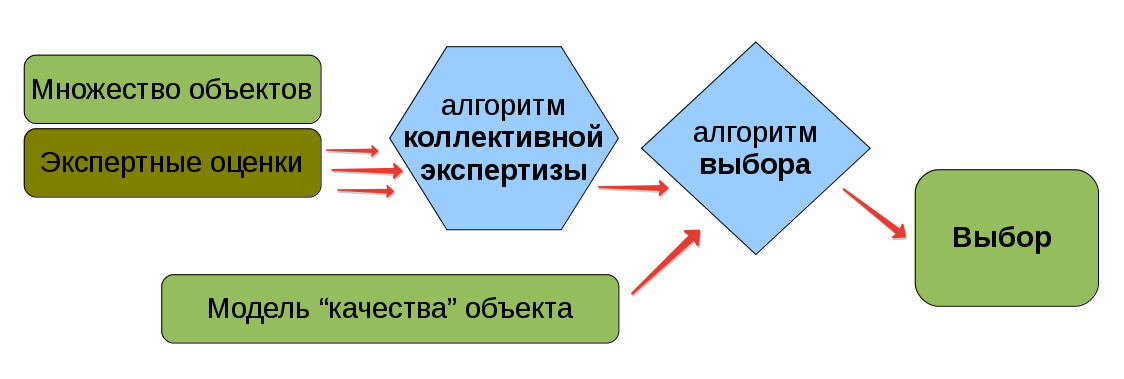
\includegraphics[width=0.8\linewidth]{./pic/globalscheme}
 	\begin{columns}
 		\column{0.45\textwidth}
 			Есть $n$ объектов, у каждого объекта % составителем методологии выбрано
 			есть $m$ нечётких параметров: 
			\\ \vspace*{2mm}
 			$\tilde x_{ij} \in X$, {\footnotesize $i = 1 \ldots n$, $j = 1 \ldots m$} 
 			\\ \vspace*{3mm}
 			$x_{ij} \in X$ -- их значения (неизвестны), где $X$ --  числовое множество. %некое выпуклое подмножество действительной оси
 		\column{0.55\textwidth}
 			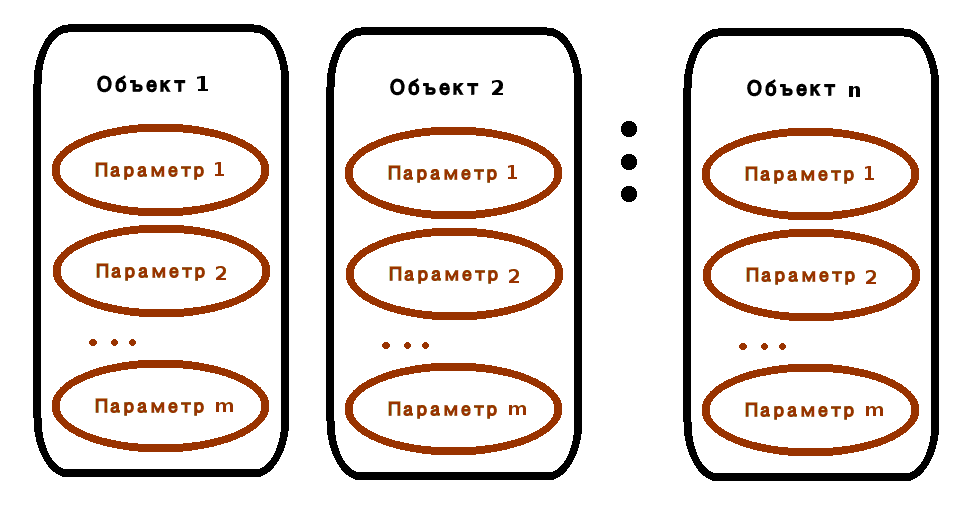
\includegraphics[width=1.0\linewidth]{./pic/theobjects}
 	\end{columns}
 	
        \hspace{20mm} { \small \tikz { \node  (n1) { \light{монотонна и задана заказчиком экспертизы}  }; } }
	 $x_i = \tikz[baseline] { \node[anchor=base, fill=green!20] (t1) {$f$}; } (x_{i1}, ..., x_{im})$ -- <<качество>> объектов.
	\begin{tikzpicture}[overlay]
	    \path[->] (n1.west) edge  (t1.north east);
	\end{tikzpicture}

	\vspace*{1mm}
	\begin{columns}
		\column{0.60\textwidth}
		Экспертные оценки -- это распределения 
		{\large \begin{center} \hspace{-20mm}  $\{ \p_{ij}(x_{ij}) \}_r$ \end{center} }
		{\footnotesize где $i = 1 \ldots n$ -- номер объекта, $j = 1 \ldots m$, -- номер параметра, $r = 1 \ldots R$ -- номер эксперта}.  
		\column{0.40\textwidth}
		\begin{center}
		    \vspace*{-4mm}
		 %   {\small Примеры оценок:}
		    {\scriptsize \light{Примеры оценок: значения $\p(x)$ показаны цветом, $x \in \setTen$}}
		    \\ \vspace*{2mm}
		     \resizebox{1.0\linewidth}{!}{\showevDisplayFullScale{./pic/chapter01-tech01.dat}}
		\end{center}
	\end{columns}
 	
\end{frame} %===========================

\begin{frame}{Пример формирования <<качества>> объекта}
	\begin{center}
		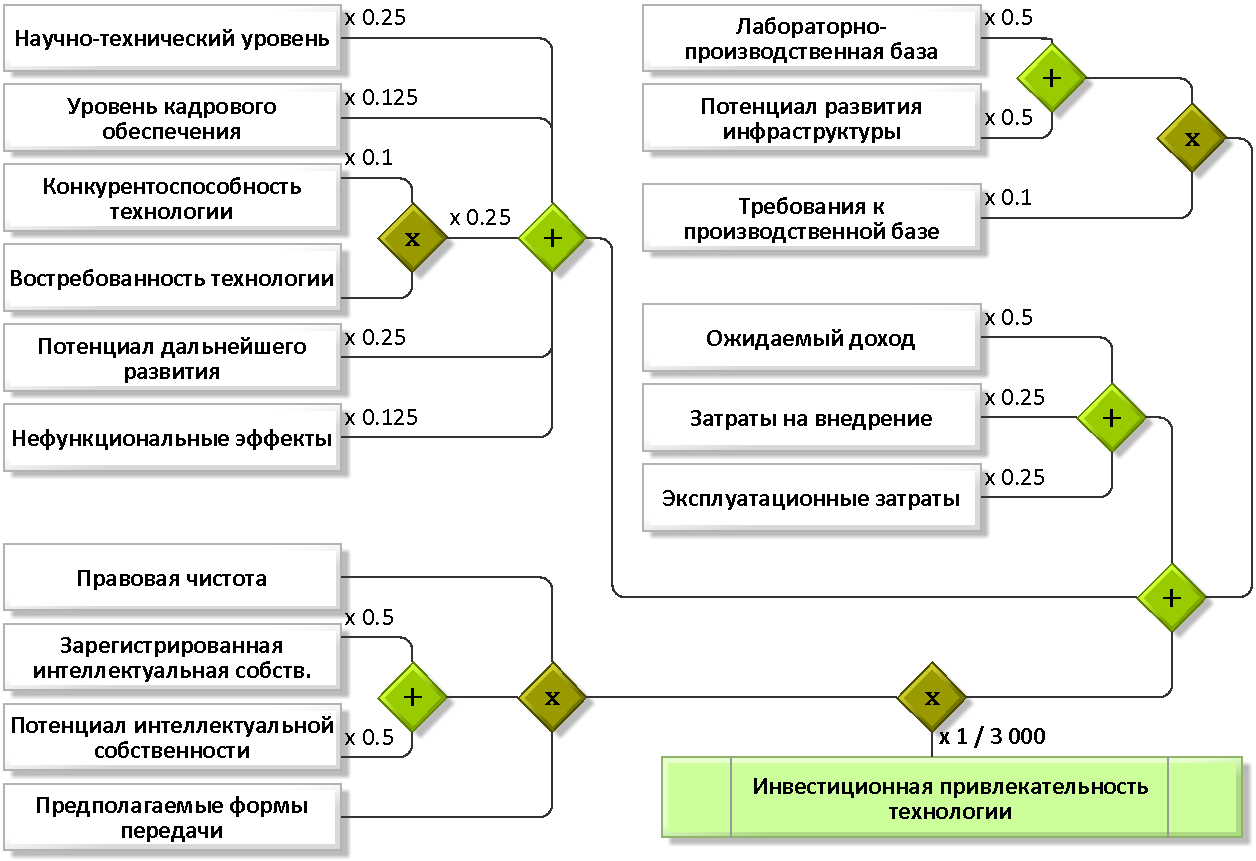
\includegraphics[width=1.0\linewidth]{./pic/schemeF2}
	\end{center}
\end{frame} %===========================

\begin{frame}{Задача оптимального выбора объектов}
	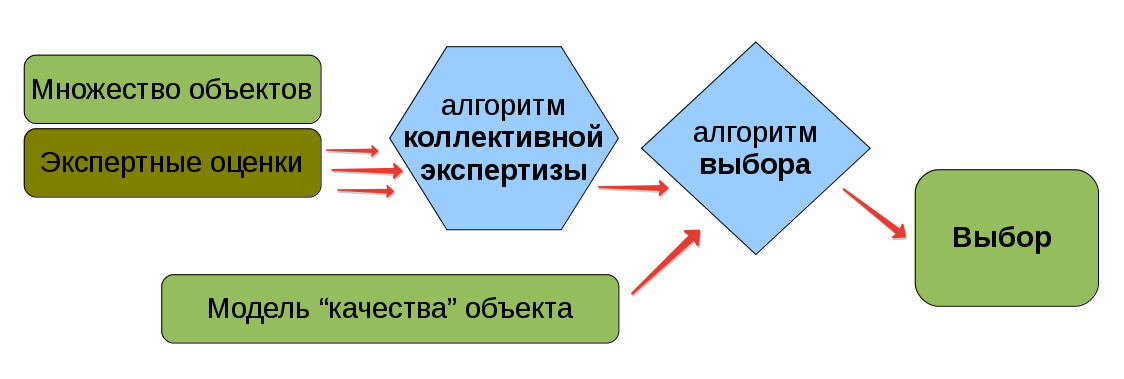
\includegraphics[width=0.8\linewidth]{./pic/globalscheme}
\end{frame} %===========================


\end{document}
